\documentclass[12pt]{article}

%%%  PAGE DIMENSIONS
\usepackage[frenchb]{babel}
\usepackage{geometry} 			
\geometry{a4paper, left=20mm, right=20mm, bottom=25mm, top=25mm} 				
\setlength{\parskip}{0.5em}					% Espace entre les paragraphes

%%%  PACKAGES
\usepackage{booktabs} 			
\usepackage{array} 				
\usepackage{verbatim} 			
\usepackage{subfig} 			
\usepackage{graphicx}			
\graphicspath{ {images/} }		
\usepackage[utf8]{inputenc}
\usepackage[T1]{fontenc}
\usepackage{listings}			
\usepackage{color}				
\usepackage{hyperref}   

%%% USER COLORS
\definecolor{darkGreen}{RGB}{0,0.6,0}
\definecolor{gray}{RGB}{0.5,0.5,0.5}
\definecolor{mauve}{RGB}{0.58,0,0.82}
\definecolor{pblue}{rgb}{0.13,0.13,1}
\definecolor{pgreen}{rgb}{0,0.7,0}
\definecolor{pred}{rgb}{0.9,0,0}
\definecolor{pgrey}{rgb}{0.46,0.45,0.48}

%%% CODE STYLE (\lstinputlisting{stcFile.cpp} ou \begin{lstlisting} et \end{lstlisting}

%%% JAVA STYLE
\lstdefinestyle{Java}
{
  language=Java,  
  inputencoding=utf8,
  frame=single,
  showspaces=false,
  showtabs=false,
  breaklines=true,
  showstringspaces=false,
  breakatwhitespace=true,
  commentstyle=\color{pgreen},
  keywordstyle=\color{pblue},
  stringstyle=\color{pred},
  basicstyle=\fontsize{9}{11}\ttfamily,
  numbers=left,
  numbersep=5px,
  numberstyle=\tiny\color{pgrey},
  stepnumber=1,
  tabsize=2
}

%%% XML Style
\lstdefinestyle{XML}
{  
  inputencoding=utf8,
  language=XML,
  frame=lines,
  showspaces=false,
  showtabs=false,
  breaklines=true,
  showstringspaces=false,
  breakatwhitespace=true,
  commentstyle=\color{pgreen},
  keywordstyle=\color{pblue},
  stringstyle=\color{pred},
  basicstyle=\fontsize{9}{11}\ttfamily,
  numbers=left,
  numbersep=5px,
  numberstyle=\tiny\color{pgrey},
  stepnumber=1,
  tabsize=2
}

%%% JSON Style
\lstdefinestyle{JSON}
{
  inputencoding=utf8,
  frame=lines,
  showspaces=false,
  showtabs=false,
  breaklines=true,
  showstringspaces=false,
  breakatwhitespace=true,
  comment=[l]{:},
  commentstyle=\color{black},
  keywordstyle=\color{pblue},
  string=[s]{"}{"},
  stringstyle=\color{pblue},
  basicstyle=\fontsize{9}{11}\ttfamily,
  numbers=left,
  numbersep=5px,
  numberstyle=\tiny\color{pgrey},
  stepnumber=1,
  tabsize=2
}

\lstdefinestyle{BASH}
{
  inputencoding=utf8,
  frame=single,
  showspaces=false,
  frameround=tttt,
  showtabs=false,
  breaklines=true,
  showstringspaces=false,
  breakatwhitespace=true,
  comment=[l]{:},
  commentstyle=\color{black},
  keywordstyle=\color{pblue},
  string=[s]{"}{"},
  stringstyle=\color{pblue},
  numbersep=5px,
  numberstyle=\tiny\color{pgrey},
  stepnumber=1,
  tabsize=2
}

% Setup pour les liens
\hypersetup{
    bookmarks=true,         
    unicode=false,          
    pdftoolbar=true,        
    pdfmenubar=true,        
    pdffitwindow=false,    
    pdfstartview={FitH},    
    pdftitle={My title},    
    pdfauthor={Author},    
    pdfsubject={Subject},  
    pdfcreator={Creator},  
    pdfproducer={Producer}, 
    pdfkeywords={keyword1, key2, key3}, 
    pdfnewwindow=true,      
    colorlinks=true,       
    linkcolor=black,         
    citecolor=green,        
    filecolor=magenta,      
    urlcolor=blue          
}

%%%  HEADERS & FOOTERS
\usepackage{fancyhdr} 
\pagestyle{fancy} 
\renewcommand{\headrulewidth}{1pt}
\renewcommand{\footrulewidth}{1pt}
\lhead{
\includegraphics[height=20px]{logo}}\chead{}\rhead{STI - Labo 2}
\lfoot{M. Chatelan \& L. Lassalle}\cfoot{}\rfoot{\thepage}

%%% NEW COMMANDS %%%		\newcommand{name}[num]{definition{#1}} -> \name{toto}
\newcommand{\ang}[1]{\emph{#1}}				
\newcommand{\mail}[1]{{#1}@heig-vd.ch}

%%% SETTINGS %%%
\setlength\parindent{0pt} 		% Taille de l'indentation

%%% TITLE
\begin{titlepage}
\title
{
  \Huge{STI - Projet}\\
  \vspace{1cm}
  \large{Modélisation de menaces}
  \vspace{2cm} \\
    
\includegraphics[width=350px]{wechatinsecure}    
        \vspace{1cm} \\
\large{vers}
  \vspace{1cm} \\
  
\includegraphics[width=350px]{wechatsecure}    
  \vspace{6cm} \\
}

\author{Matthieu Chatelan \& Loan Lassalle} 
\date{\today}

\end{titlepage}

\begin{document}

\maketitle
\thispagestyle{empty}

\clearpage
\tableofcontents
\listoffigures
\setcounter{page}{1}        % Set page numbering to begin on this page
\clearpage

\section{Introduction}
Le but de ce document est de fournir une analyse de menaces auquels notre programme WeChat est exposé.
Premièrement, une description du système est donnée fournissant ainsi une meilleure compréhension des
différents composants de ce dernier, les différents rôles mis à disposition ou encore les biens 
qui seront à protéger.

Ensuite, une analyse des différentes sources de menaces auquels notre programme sera exposé. Les différentes
sources potentielles sont énumérées ainsi que les compétences requises pour effectuer chacunes de ces attaques.

Finalement, plusieurs scénarios d'attaques seront donnés ainsi que les contremesures appropriées à mettre
en place afin de les contrer.

%%%%%%%%%%%%%%%%%%%%%%%%%%%%%%%%%%%%%%%%%%%%%%%%%%%%%%%%%%%%%%%%%%%%%%%%%%%%%%%%%%%%%%%%%%%%%%
%%%%%%%%%%%%%%%%%%%%%%%%%%% DESCRIPTION SYSTEME %%%%%%%%%%%%%%%%%%%%%%%%%%%%%%%%%%%%%%%%%%%%%%
%%%%%%%%%%%%%%%%%%%%%%%%%%%%%%%%%%%%%%%%%%%%%%%%%%%%%%%%%%%%%%%%%%%%%%%%%%%%%%%%%%%%%%%%%%%%%%
\section{Description du système}
\subsection{Objectifs du système}

Les objectifs fixés du système étaient de développer une application web permettant d'envoyer  et de reçevoir des messages textes entre collaborateurs au sein d'une entreprise. Le protocole de transmission SMTP ne devait pas être utilisé pour cette application.

Cette application serait par exemple utilisée entre employés d'une entreprise de développement de logiciels.

\subsection{Exigences du système}

Lors du développement de l'application, plusieurs contraintes ont été fixées par le client dans le cahier des charges. Dans les sous sections ci-dessous, ces dernières sont décrites et expliquées. 

\subsubsection{Exigences technologiques}
Pour développer l'application, les différentes technologies suivantes ou contraintes ont dû être prises en compte :

\begin{itemize}
\item PHP
\item SQLite
\item Doit fonctionner sur l'environnement CentOS fournis
\end{itemize}

\subsubsection{Exigences fonctionnelles}

L'application devait être en mesure proposer deux rôles différents soit \textbf{collaborateur}, soit \textbf{administrateur}. De plus, un mécanisme d'authentification simple (utilisateur - mot de passe) doit permettre d'accéder aux fonctionnalités. Pour pouvoir se connecter, un utilisateur doit être définit comme étant "actif".

Une navigation aisée via des liens ou des boutons devait être mise en place.

\newpage
Un \textbf{collaborateur} doit pouvoir effectuer les actions suivantes : 

\begin{enumerate}
\item Lire les messages reçus sous forme de liste triée par ordre de date de réception avec plusieurs informations tels que :

\begin{itemize}
\item[--] la date de réception
\item[--] l'expéditeur
\item[--] le sujet
\item[--] un bouton permettant de répondre au message (avec le sujet directement définit)
\item[--] un bouton permettant de supprimer le message
\item[--] un bouton permettant d'ouvrir un message et de voir le contenu du corps 
\end{itemize} 

\item Ecrire des messages à l'attention d'un autre utilisateur. Les informations suivantes doivent être fournies :

\begin{itemize}
\item[--] destinataire (unique)
\item[--] sujet
\item[--] corps du message
\end{itemize} 

\item Changer le mot de passe de l'utilisateur connecté.

\end{enumerate}

Un \textbf{administrateur} doit pouvoir effectuer les actions suivantes : 

\begin{enumerate}
\item Avoir les mêmes actions qu'un collaborateur

\item Ajouter, modifier ou supprimer un utilisateur, représenté par les attributs suivants : 

\begin{itemize}
\item[--] Un login (non modifiable)
\item[--] Un mot de passe (modifiable)
\item[--] Une validité actif/inactif (modifiable)
\item[--] Un rôle (modifiable)
\end{itemize} 

\end{enumerate}

\subsubsection{Exigences sécuritaires}
Une authentification était demandée. Cette dernière ne devait pas permettre l'accès à toute autre page que celle de login lorsque l'utilisateur n'est pas authentifié.

Lors du développement initial, aucunes autre mesures de sécurité n'étaient demandées. De ce fait, aucunes protections contre des attaques XSS, CSRF, SQL Injection ou autre n'ont été mises en places.

Néanmoins, les mots de passes n'étaient pas stockés en clair dans la base de donnée, mais sous forme de hash salé pour empêcher une attaque par rainbow table sur ces derniers.

\newpage
\subsection{Constitution du système}

Le système développé comprenait plusieurs acteurs et processus ainsi qu'une base de donnée centrale. Dans le diagramme de flux de données de l'application (Figure \ref{flux}), un acteur est représenté par un rectangle alors qu'un processus est représenté par un cercle.

On notera que tous les processus qui se situent au dessus de la base de données dans le diagramme (5 au total) sont des processus que les deux acteurs peuvent utiliser. En revanche, les 3 processus au dessous de la base de données sont des processus réservés aux administrateurs.

Lellipse traitillée en orange représente la frontière de confiance de l'application. Cela signifie que nous considérons que les communications entres processus et la base de données sont sécurisés. Toutes entrées utilisateur doivent être contrôlés avant de pénétrer cette zone de confiance.

\begin{figure}[h]
 	\center
	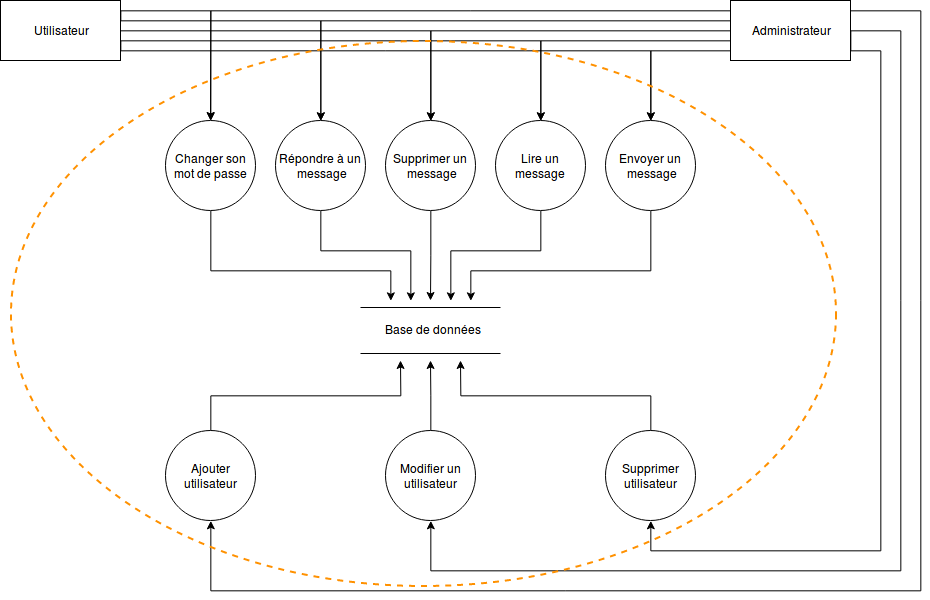
\includegraphics[width=480px]{diagram}
 	\caption{Diagramme de flux de données de l'application} 
 	\label{flux}	
\end{figure}


\subsection{Biens}
Les biens à protéger sont multiples dans une telle application. Ci-dessous, une liste non exhaustive de ces derniers

\begin{itemize}
\item Les messages 
\item Les comptes utilisateurs (leurs mots de passes)
\item L'accès à l'administration des comptes
\end{itemize}

%%%%%%%%%%%%%%%%%%%%%%%%%%%%%%%%%%%%%%%%%%%%%%%%%%%%%%%%%%%%%%%%%%%%%%%%%%%%%%%%%%%%%%%%%%%%%%
%%%%%%%%%%%%%%%%%%%%%%%%%%% SOURCES MENACES %%%%%%%%%%%%%%%%%%%%%%%%%%%%%%%%%%%%%%%%%%%%%%%%%%
%%%%%%%%%%%%%%%%%%%%%%%%%%%%%%%%%%%%%%%%%%%%%%%%%%%%%%%%%%%%%%%%%%%%%%%%%%%%%%%%%%%%%%%%%%%%%%
\newpage
\section{Sources de menaces}

\subsection{Liste des acteurs}
\begin{tabular}{| l | l | l | c |}
  \hline			
  \textbf{Initiateur} & \textbf{Motivations} & \textbf{Cible(s)} & \textbf{Potentialité} \\
  \hline
  Utilisateur & Fun, Revanche, Curiosité & Tout éléments accessibles & Haute \\
  Administrateur & Revanche, Curiosité & Tout éléments accessibles & Moyenne \\  
  Concurrent & Secrets d'entreprise & Base de données & Moyenne \\
  Hackers & Gloire, Argent, Destruction & Tout éléments accessibles & Faible \\
  Cyber-criminel & Vol d'informations, Spam, DDoS & Base de données & Faible \\
  Etat & Vol d'informations, Profit & Tout éléments accessibles & Faible \\
  \hline  
\end{tabular}
\\

Parmi les différents initiateurs décrits ci-dessus, les utilisateurs représentent la plus grande menace et la menace la plus probable d'arriver. En effet, comme le programme est destiné à un usage interne à l'entreprise, a priori seuls les employés y auront accès.

Un administrateur est par défaut une source de menace implicite car ce dernier à un accès total à l'application. Il sera dans notre cas en mesure d'ajouter des utilisateurs ou d'en supprimer, ou encore de les désactiver ou changer leur rôle. Si il a un accès à la base de données, il aura accès à toutes les informations contenues dans cette dernière.

\subsection{Pyramide des acteurs}

\begin{figure}[h]
 	\center
	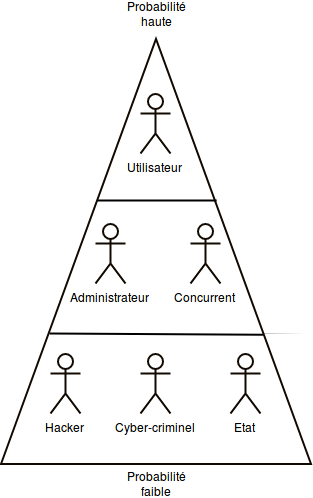
\includegraphics[width=200px]{pyramid}
 	\caption{Pyramide des sources de menace} 
 	\label{flux}	
\end{figure}


%%%%%%%%%%%%%%%%%%%%%%%%%%%%%%%%%%%%%%%%%%%%%%%%%%%%%%%%%%%%%%%%%%%%%%%%%%%%%%%%%%%%%%%%%%%%%%
%%%%%%%%%%%%%%%%%%%%%%%%%%% SCENARIOS D'ATTAQUE %%%%%%%%%%%%%%%%%%%%%%%%%%%%%%%%%%%%%%%%%%%%%%
%%%%%%%%%%%%%%%%%%%%%%%%%%%%%%%%%%%%%%%%%%%%%%%%%%%%%%%%%%%%%%%%%%%%%%%%%%%%%%%%%%%%%%%%%%%%%%
\newpage
\section{Scénarios d'attaques}

Dans cette section, plusieurs scénarios d'attaque sont décrits. Grâce à ces scénarios, il est possible d'imaginer les différents points vulnérables de l'application et ainsi permet de mettre en place des contremesures appropriées.

Ces différents scénarios sont regroupés par impacte et non par vulnérabilité. Il se peut qu'un impacte soit causé par de multiples failles de sécurité.

\begin{tabular}{| c | p{5.5cm} | p{5.5cm} | l |}
  \hline			
  \textbf{\# }& \textbf{Impacte} &\textbf{ Source de menace } & \textbf{Bien ciblé} \\
  \hline  
  \ref{1} & Perte de confidentialité & Utilisateur, Concurrent, Hacker, Cyber-criminel & BDD \\
    \hline  
  \ref{2} & Perte de disponibilité & Utilisateur, Concurrent, Hacker, Cyber-criminel & Tout élément actif \\
    \hline  
  \ref{3} & Perte d'intégrité & Hacker, Concurrent & BDD \\
  \hline  
 \ref{5} & Accès à des ressources non autorisées & Utilisateur, Hacker, Concurrent & Application, BDD \\
  \hline 
\end{tabular}
\\

Les différents scénarios d'attaques et leurs sources de menaces dépendent de comment l'application de chat est déployée et de comment elle est utilisée par les employés. En effet, si l'application est accessible par l'extérieur de l'entreprise, il sera facile pour des intervenants externes tels que des cyber-criminels ou des hackers d'accèder directement aux biens.

En revanche, si l'application est déployée sur un réseau local non accessible par l'extérieur, un attaquant externe devra s'introduire dans le réseau avant de pouvoir attaquer l'application et accèder aux biens. De l'ingénierie sociale peut être utilisée pour inciter un employer à visiter un lien ou à installer une application vulnérable.

\subsubsection{Perte de confidentialité} \label{1}
Dans ce scénario d'attaque, les différents acteurs listés en tant que source de menace tenteront d'accèder à des informations qui ne leurs sont pas destinées causant ainsi une perte de confidentialité. 

Pour parvenir à ses fins, un attaquant pourra essayer de multiples vecteurs d'attaque tels que : 

\begin{itemize}
\item Manipulation de l'URL
\item Injection SQL dans les divers champs de saisie vulnérables
\item Utilisation d'une faille de XSS stocké afin de récupérer des cookie de session
\end{itemize}

Sans des connaissances poussées en informatique, on pouvait très rapidement remarquer que lors de la lecture d'un message, l'id de ce dernier était donnée dans l'URL. Etant donné qu'aucunes vérification n'était faite du côté serveur pour s'assurer que la personne lisant le message était bien le destinataire de ce dernier, il était possible d'écrire un script python qui testait de manière incrémentale l'accès à tous les message en incrémentant l'id de ce dernier. Si en réponse une erreur 404 est obtenue, on sait que le message n'existe pas. En revance, si un code 200 est retourné, on sait qu'un message existe et on peut automatiquement l'extraire et le stocker dans un fichier ou le parser afin de tenter de trouver des informations confidentielles tels que des adresses mail ou des mots de passes.

Avec peu de recherches sur internet et quelques tentatives, un attaquant avec de faibles connaissances sera en mesure de récupérer des données confidentielles tels que des mails ou encore des mots de passes en utilisant une injection SQL. Une fois les mots de passes récupérés, une étape de cassage hors ligne est nécessaire étant donné que mots de passes sont stocké sous forme hachée et salée.

Avec une attaque plus élaborée, cet attaquant pourrait récupérer des cookie de session en se servant d'une attaque par XSS. Pour récupérer des informations sur les conversations d'un utilisateur, une solution serait d'envoyer un message avec du code javascript en tant que sujet du message. Ce dernier sera stocké sur le serveur et lorsque l'utilisateur cible se connectera à sa boîte de réception, le code malicieux sera exécuté car les sujets sont affichés. Tous les destinataires ou sujets des messages reçus affichés par la victime peuvent être envoyés à l'attaquant (tant que notre message est toujours visible dans la liste et donc que le script est exécuté).

L'exemple de code ci-dessous à insérer dans le champ sujet du message permet de récupérer facilement tout le contenu html de la page après un délai de une seconde (pour laisser le temps aux autres informations de s'afficher dans le navigateur de la cible). Ici l'exemple ne transmet pas les informations à l'attaquand mais les affichent à la cible. 

\begin{lstlisting}[style=JAVA]
<script>
	setTimeout(() => {alert(document.documentElement.innerHTML);}, 1000);
</script>
\end{lstlisting}

\subsubsection{Perte de disponibilité} \label{2}

Ce scénario concerne la destruction d'informations par les différentes sources de menaces citées dans le tableau. Pour parvenir à ses fins, un attaquant aura plusieurs approches possibles tels que : 

\begin{itemize}
\item Manipulation de l'URL
\item Attaques XSS
\item Attaques CSRF
\item Injections SQL
\end{itemize}

Comme ennoncé précédement, comme les paramètres des actions sont passées dans l'url en clair, il serait possible pour un utilisateur de supprimer un message dont il n'est pas le destinataire légitime. En effet, tous les messages de la base de données peuvent être effacés par un seul utilisateur qui lancera un script parcourant tous les id possibles et émettant la requete de suppression pour cet id.

On pourrait imaginer une action similaire lancée par un script javascript inséré dans un corps de message (attaque XSS), permettant par exemple "l'autodestruction" du message envoyé après un certain temps après la lecture. Le script serait donc exécuté lors de l'ouverture du message, et récupérerait l'id du message dans l'URL. Après quelques secondes, on exécute la suppression de ce message en contactant le bon end-point avec cet id.

Même si une simple verification que seul le propriétaire du message peut le supprimer, un attaque par CSRF est toujours possible si aucunes autres mesures de protection ne sont mises en oeuvre. Un attaquant pourra envoyer un lien déguisé (short google URL ou autre) à la cible. Si lors du clic sur ce dernier la victime est connectée et authentifiée sur le site, l'attaquant pourra forcer la victime à supprimer un message sur son compte.

Une injection SQL peut permettre à un attaquant de complètement détruire la base de donnée (drop) ou simplement arrêter le serveur avec une commande "shutdown".

\subsubsection{Perte d'intégrité} \label{3}

Dans ce scénario d'attaque, un attaquant pourrait se servir de certaines attaques dans le but de corrompre les données présentes dans la base de données produisant ainsi une perte d'intégrité.

Si l'utilisateur utilisé pour faire la requête SQL officiellement prévue a les droits d'écriture dans la base de donées, un attaquant pourrait se servir d'une injection SQL pour effectuer plusieurs actions sur la base de données. Par exemple, au lieu de simplement lire une entrée dans la BDD, il pourrait aussi effectuer une autre action comme ajouter un utilisateur avec les droits administrateurs. De plus, il pourrait corrompre tous les messages. Dans une première phase, il pourrait récupérer les messages, puis dans un second temps les chiffrer / modifier ou les supprimer. Finalement, il pourrait renvoyer ces messages modifiés dans la base de données.

\subsubsection{Accès non autorisé à des ressources} \label{5}

Avec la version actuelle du programme, un attaquant pourrait effectuer une énumération des ressources accessibles sur le serveur web. Grâce à un programme comme dirbuster et un dictionnaire des noms de dossiers et de ressources les plus courantes, ce dernier pourra énumérer chacunes des ressources et tenter d'y accèder sans que ces dernières ne soient référencées dans les pages accessibles par les clients.

Dans le cas de cette application, un dossier \textit{docker} est à la racine du serveur web. Un utilisateur ne devrait pas avoir accès à ce dossier. Avec dirbuster, il se peut qu'un utilisateur trouve cette ressource.

%%%%%%%%%%%%%%%%%%%%%%%%%%%%%%%%%%%%%%%%%%%%%%%%%%%%%%%%%%%%%%%%%%%%%%%%%%%%%%%%%%%%%%%%%%%%%%
%%%%%%%%%%%%%%%%%%%%%%%%%%% CONTREMESURES %%%%%%%%%%%%%%%%%%%%%%%%%%%%%%%%%%%%%%%%%%%%%%%%%%%%
%%%%%%%%%%%%%%%%%%%%%%%%%%%%%%%%%%%%%%%%%%%%%%%%%%%%%%%%%%%%%%%%%%%%%%%%%%%%%%%%%%%%%%%%%%%%%%
\newpage
\section{Contremesures}

Le entrées du tableau ci-dessous reprennent les vulnérabilités énoncées dans les différents scénarios et leur font correspondre des contremesures possibles.

\begin{tabular}{| p{0.7cm} | p{7.5cm} | p{7.5cm} |}
  \hline			
  \textbf{\# } &\textbf{ Vulnérabilité }& \textbf{Contremesure} \\
  \hline  
  \ref{c1} & Manipulation de l'URL & Contrôler les entrées utilisateurs du côté serveur et utiliser des paramètres non prédictibles \\
  \hline
  \ref{c2} & Attaque XSS & Filtrer l'affichage des données stockées \\
  \hline
  \ref{c3} & Injection SQL & Utiliser des requêtes préparées \\
  \hline
  \ref{c4_1} \ref{c4_2} & Attaque CSRF & Authentification par jeton et par HTTP\_REFERER \\
  \hline
  \ref{c5} & Path Discovery & Limiter l'accès aux ressources \\
  \hline
  \ref{c6} & Bruteforce lors de l'authentification & Ralentir le processus et limiter le nombre de tentatives \\
  \hline
  \ref{c7} & Erreur d'exécution & Contrôles côté serveur \\
  \hline
  \ref{c8} & Récupération des identifiants de connexion & Utiliser le protocole HTTPS \\
  \hline
  \ref{c9} & Vol de cookie & Vérouiller la session à un seul hôte et conserver le même identifiant de session pendant un intervalle de temps donné \\
  \hline
  \ref{c10} & Manipulation d'URL & Utiliser des identifiants non prédictibles \\
  \hline
\end{tabular}\\


Parmis ces contermesures, seules les trois dernières n'ont pas été implémentées par manque de temps. Les autres mesures mises en places permettent à chaque fois de mitiger les risques énoncés dans les différents scénarios d'attaques.

\newpage

\subsection{Contremesure}\label{c1}

Afin d'éviter la manipulation d'URL et ainsi l'utilisation de fonction restreintes ou non authorisées pour certains utilisateurs, nous vérifions si les valeurs des paramètres contenus dans l'URL sont associés ou non à l'utilisateur. 

Par exemple, afin d'éviter que l'utilisateur soit capable de lire ou de supprimer n'importe quel email, nous vérifions que l'ID de l'email demandé est bien associé à l'utilisateur courant à l'aide du code suivant : 

\begin{lstlisting}[style=JAVA]
/**
 * Redirect the user if is not associated to email
 */
public function redirect_if_is_not_associate_to_user($id) {
    if ($this->get_by_id($id) === null) {
        self::$_database->deconnection();
        header('location:/wechat/home.php');
        exit;
    }
}

/**
 * Retrieves user's email
 */
public function get_by_id($id) {
    $user_id = self::$_user->get_id();
    $query = "SELECT date, 
                    uSender.username AS 'from', 
                    uReceiver.username AS 'to', 
                    subject, 
                    body 
                    FROM mails 
                    LEFT JOIN users AS uSender ON mails.idSender = uSender.id 
                    INNER JOIN users AS uReceiver ON mails.idReceiver = uReceiver.id 
                    WHERE mails.id=:id 
                    AND idReceiver=:user_id;";
    $parameters = array(new Parameter(':id', $id, PDO::PARAM_INT),
                        new Parameter(':user_id', $user_id, PDO::PARAM_INT));
    $array = self::$_database->query($query, $parameters);

    return count($array) >= 1 ? $array[0] : null;
}
\end{lstlisting}

Cette technique a aussi été mise en place pour l'édition ou la suppression d'un utilisateur. Cela permet d'éviter que l'administrateur courant puisse supprimer son propre compte.
Cette contremesure a été mise en place dans les fichiers suivant :

\begin{itemize}
\item controllers/delete\_mail.php
\item controllers/delete\_user.php
\item controllers/read\_mail.php
\item read\_mail.php
\item write\_mail.php
\end{itemize}

\newpage
\subsection{Contremesure}\label{c2}

Afin d'éviter les attaques XSS, nous avons mis en place la fonction \textit{htmlentities}. Cette fonction permet de convertir tous les caractères éligibles en entités HTML. Ce qui permet d'éviter d'éxecuter du code non autorisé.

\begin{lstlisting}[style=JAVA]
<td>'.htmlentities($mail['from'], ENT_QUOTES | ENT_HTML5, 'UTF-8').'</td>
<td>'.htmlentities($mail['subject'], ENT_QUOTES | ENT_HTML5, 'UTF-8').'</td>
\end{lstlisting}

Nous l'avons mis en place lorsque l'application Web affiche des informations stockées dans la base de données ou tout éléments provenant de la saisie utilisateur. Ainsi l'application Web n'est pas vulnérable aux attaques XSS stockées.

Cette contremesure a été mise en place dans les fichiers suivant :

\begin{itemize}
\item home.php
\item manage\_user.php
\item read\_mail.php
\item write\_mail.php
\end{itemize}

Une attaque XSS réfléchie n'est pas possible sur le site. Aucuns paramètres passés par l'url ne sont directement affichés par le navigateur et donc aucune injection de code n'est possible.

\newpage
\subsection{Contremesure}\label{c3}

Afin d'éviter les injections SQL, nous avons mis en place des requêtes préparées. Elles permettent d'interpréter correctement les différents types des paramètres d'une requête . Pour être plus précis, si une requête utilise une chaîne de caractères comme paramètre, elle l'englobera de guillemets afin de tranformer toute la valeur du paramètre en chaîne de caractères et ceci afin d'éviter les injections SQL.

Voici un extrait de code métant en place cette contremesure : 

\begin{lstlisting}[style=JAVA]
/**
 * Get the result of a query
 */
public function query($sql, $parameters) {
    if (!isset($this->_pdo)) {
        $this->connection();
    }

    $stmt = $this->_pdo->prepare($sql);
    
    if (isset($parameters)) {
        foreach($parameters as $parameter) {
            $stmt->bindParam($parameter->get_name(), $parameter->get_value(), $parameter->get_pdo_type());
        }
    }

    $stmt->execute();

    return $stmt->fetchAll(PDO::FETCH_ASSOC);
}
\end{lstlisting}

Cette technique permet aussi d'éviter que l'application Web crash lors de l'utilisation de requête avec des paramètres ne correspondant pas au type attendu.
Cette contremesure a été mise en place dans les fichiers suivant :

\begin{itemize}
\item models/Blacklist.php
\item models/Database.php
\item models/Mail.php
\item models/Role.php
\item models/User.php
\end{itemize}

\newpage
\subsection{Contremesure}\label{c4_1}

Afin d'éviter les attaques CSRF, nous avons mis en place l'authentification par jeton. Cette technique est mise en place sur une page d'origine et une page de destination.
Dans notre application, nous générons 2 jetons au sein de la page d'acceuil pour accéder au liens de suppression d'email et d'utilisateurs.

\begin{lstlisting}[style=JAVA]
// Generates token for link authentication
$token_mail = Utils::get_instance()->random_str(32);
$_SESSION['token_mail'] = $token_mail;

$token_user = Utils::get_instance()->random_str(32);
$_SESSION['token_user'] = $token_user;
\end{lstlisting}

Puis au sein des page de destination, dans notre cas les pages de suppression, nous vérifions si les jetons générés et enregistrés dans la session précédement sont égales à ceux contenu dans l'URL.

\begin{lstlisting}[style=JAVA]
$token = isset($_SESSION['token_mail']) && isset($token) ? $token : "";

if ($_SESSION['token_mail'] === $token) {
    // Delete mail
}

// Redirect to home
\end{lstlisting}

Cette technique se repose sur la génération d'une chaîne de caratères aléatoire. C'est pourquoi il est indispensable de veiller à rendre la génération de jeton non prédictible. Nous avons implémenté cette technique uniquement pour les actions de suppression car s'est une action à haut risque et qu'elle produit un changement rapide de l'interface et très peu visible par l'utilisateur. 
Cette contremesure a été mise en place dans les fichiers suivant :

\begin{itemize}
\item controllers/delete\_mail.php
\item controllers/delete\_user.php
\item read\_mail.php
\end{itemize}

\newpage
\subsection{Contremesure}\label{c4_2}

Afin d'éviter les attaques CSRF, nous avons aussi mis en place une vérification du referer header. 

\begin{lstlisting}[style=JAVA]
/**
 * Checks if is correct file origin
 */
public function redirect_if_is_not_correct_file_origin($files_origin) {
    $http_referer_file = substr($_SERVER['HTTP_REFERER'], strrpos($_SERVER['HTTP_REFERER'], '/') + 1);
    $ask_pos = strrpos($http_referer_file, '?');

    if ($ask_pos !== false) {
        $http_referer_file = substr($http_referer_file, 0, $ask_pos);
    }
    
    foreach ($files_origin as $file_origin) {
        if ($http_referer_file === $file_origin) {
            return;
        }
    }

    header('location:/wechat/home.php');
    exit();
}
\end{lstlisting}

Bien que cette sécurité est redondante par rapport à la vérification de jeton, nous avons décidé d'implémenter les 2 techniques afin de montrer les différentes possibilités pour éviter les attaques CSRF. Cependant, il est possible de modifier la valeur du HTTP\_REFERER, c'est pour cette raison que cette technique est controversée.
Cette contremesure a été mise en place dans les fichiers suivant :

\begin{itemize}
\item controllers/delete\_mail.php
\item controllers/delete\_user.php
\item controllers/login.php
\item controllers/send\_mail.php
\item controllers/update\_password.php
\item controllers/update\_user.php
\item models/Utils.php
\end{itemize}

\newpage
\subsection{Contremesure}\label{c5}

Afin d'éviter l'accès à certaines ressources du site Internet, nous avons mis en place des directives au sein du fichier de configuration du serveur Apache (/etc/httpd/conf/httpd.conf) qui s'appliquent au répertoire et sous-répertoires de notre application Web.

\begin{lstlisting}[style=JAVA]
#
# "/var/www/html/wechat"
#
<Directory /var/www/html/wechat/>
    AllowOverride None
    Options -Indexes
    ErrorDocument 403 /wechat/errors/forbidden.php
    <FilesMatch "\.php|\.css|\.html">
        Allow from All
    </FilesMatch>
</Directory>

#
# "/var/www/html/wechat/*/"
# Subdirectories
#
<Directory /var/www/html/wechat/\*/>
    AllowOverride None
    Deny from All
</Directory>

#
# "/var/www/html/wechat/css/"
#
<Directory /var/www/html/wechat/css/>
    AllowOverride None
    Allow from All
</Directory>

#
# "/var/www/html/wechat/controllers/"
#
<Directory /var/www/html/wechat/controllers/>
    AllowOverride None
    Allow from All

    # TODO: Remove comments if you are in environment production
    # <Files init.php>
    #     Deny from All   
    # </Files>
</Directory>

#
# "/var/www/html/wechat/errors/"
#
<Directory /var/www/html/wechat/errors/>
    AllowOverride None
    Allow from All
</Directory>

#
# "/var/www/html/wechat/models/"
#
<Directory /var/www/html/wechat/models/>
    AllowOverride None
    Allow from All
</Directory>
\end{lstlisting}

La première directive permet d'autoriser l'accès à tous les fichiers d'extension php, css et html. Elle permet aussi de ne pas renvoyer un listing formaté du répertoire et de rediriger toutes les requêtes dont l'accès est non autorisée vers la page d'acceuil ou d'authentification. 
La deuxième directive définit le blocage de l'accès au sous-répertoires de l'application Web.
Les quatres dernières directives sont utilisées pour autoriser uniquement l'accès aux ressources des différents répertoires définits.
Cette contremesure a été mise en place dans le fichier suivant :

\begin{itemize}
\item httpd.conf
\end{itemize}

\newpage
\subsection{Contremesure}\label{c6}

Afin d'éviter les attaques par bruteforce, nous avons bloqué l'authentification de l'utilisateur en insérant son adresse IP dans une liste noire d'adresse IP une fois un nombre trop élevé de tentatives effectuées.

\begin{lstlisting}[style=JAVA]
// Get attempt of IP address of current user
$attempt = Blacklist::get_instance()->get_attempt();
$is_blacklisted = isset($attempt) && $attempt >= Blacklist::ATTEMPTS_MAX;

if (!$is_blacklisted) {
    
    // Authenticate the user
    if ($is_correct_username && $is_correct_password) {
        if (isset($attempt)) {
            Blacklist::get_instance()->increment_attempt();
        } else {
            Blacklist::get_instance()->set();
        }

        $is_error = !Authentication::get_instance()->is_authenticated($username, $password);
    }
}

// Redirect the user after authentication
if (isset($is_error) && $is_error) {
    header('location:/wechat/index.php?is_error=true');
} else if ($is_blacklisted) {
    Blacklist::get_instance()->max_attempt();
    header('location:/wechat/errors/attempts.html');
} else {
    Blacklist::get_instance()->reset();
    header('location:/wechat/home.php');
}
\end{lstlisting}

Nous avons préféré un blocage par rapport à l'adresse IP plutôt que par rapport au nom d'utilisateur. Cette technique évite qu'un attaquant ne bloque l'accès au site Internet de tous les comptes utilisateurs. Etant donné la simplicité de notre application Web, nous avons décidé de bloquer l'authentification de l'utilisateur au bout de 4 essais. Il serait intéressant, au bout de 4 essais, de bloquer l'adresse IP de l'utilisateur un temps donné. Cela permettrait aux utilisateurs non attentifs de pouvoir se connecter à nouveau sans contacter l'administrateur du site Internet. 

Bien sur une fois cette technique mise en place, il faudrait augmenter le temps d'attente si l'utilisateur échoue à nouveau son authentification. Cette technique ralentirait d'avantages les attaques par bruteforce. 

Puis comme dernier rempart de sécurité, il faudrait bloquer définitivement l'adresse IP de l'utilisateur lorsqu'il a trop échoué l'authentification. Il lui serait possible, via un formulaire exempt de vulnérabilités, de faire une demande de suppression de restriction à l'administrateur du site Internet.

Pour terminer, il serait recommandé de mettre en place une politique de mot de passe complexe. Il faudrait par exemple,  autoriser uniquement l'utilisation de mot de passe contenant des lettres minuscules et majuscules, des chiffres, des symboles, éviter les répétitions de mots et l'utilisation d'informations personnelles. 

Bien évidemment, toutes ces techniques ne rendent pas impossible les attaques bruteforce mais ralentissent énormément le processus.

Cette contremesure a été mise en place dans les fichiers suivant :

\begin{itemize}
\item controllers/login.php
\end{itemize}

\newpage
\subsection{Contremesure}\label{c7}

Afin d'éviter les erreurs d'exécution, nous avons mis en place la vérification des saisies utilisateurs. Cette technique consiste à vérifier la longueur des chaînes de caractères, a quel domaine mathématique appartient les valeurs numériques ou encore si la valeur est représentable dans le type de destination.

\begin{lstlisting}[style=JAVA]
if (isset($from) && isset($to) && isset($subject) && isset($body)) {
    $len_from = strlen($from);
    $is_correct_from = $len_from >= Database::USERNAME_MIN && 
                    $len_from <= Database::USERNAME_MAX;
                            
    $len_to = strlen($to);
    $is_correct_to = $len_to >= Database::USERNAME_MIN && 
                    $len_to <= Database::USERNAME_MAX;

    $len_subject = strlen($subject);
    $is_correct_subject = $len_subject >= Database::PHP_STR_MIN && 
                    $len_subject <= Database::PHP_STR_MAX;
                            
    $len_body = strlen($body);
    $is_correct_body = $len_body >= Database::PHP_TEXT_MIN && 
                    $len_body <= Database::PHP_TEXT_MAX;

  if ($is_correct_from &&  $is_correct_to && $is_correct_subject && $is_correct_body) {
    // Do something with these correct input
  }
} else {
 // Input incorrect
}
\end{lstlisting}

Cette contremesure a été mise en place dans les fichiers suivant :

\begin{itemize}
\item controllers/login.php
\item controllers/send\_mail.php
\item controllers/update\_password.php
\item controllers/update\_user.php
\item write\_mail.php
\end{itemize}

\newpage
\subsection{Contremesure}\label{c8}

Afin d'éviter que les identifiants de connexion d'un utilisateur ne passent en clair sur le réseau, il serait nécessaire de mettre en place une connexion chiffrée à l'application Web. Cette technique garantirait la confidentialité des données échangées avec le serveur empéchant un attaquant de se positionner en MITM.

Nous avons décidé de ne pas mettre en place cette technique au sein de l'application Web parce qu'elle n'est pas destiné à un environnement de production et que nous ne voulions pas perdre de temps à sa mise en place.

Un certificat peut être obtenu relativement simplement avec Let's Encrypt si le site internet à un nom de domaine associé.

\subsection{Contremesure}\label{c9}

Afin d'éviter le vol de session, il serait utile de mettre en place un vérouillage de la session par hôte. En utilisant l'adresse IP et le User Agent de l'utilisateur, nous pouvons ainsi éviter cette attaque. Afin d'ajouter une couche de sécurité, nous pourrions mettre en place une regénération de session. Rendre la session obsolète après une durée déterminée permettrait d'empêcher l'utilisation d'une session volée ad vitam eternam.
Nous avons essayé de le mettre en place mais nous n'y sommes pas arrivés. Nous pensons que le problème provient de l'architecture de notre application Web. 

Toutefois, nous avons trouvé un exemple d'implémentation sur le site suivant :

\url{http://blog.teamtreehouse.com/how-to-create-bulletproof-sessions}

\subsection{Contremesure}\label{c10}

Afin d'éviter la manipulation d'URL, nous aurions pu utiliser des identifiants non prédictibles pour  effectuer des actions sur les emails et les utilisateurs. Cette technique se serait appuyée sur la génération d'une empreinte de l'objet afin d'effectuer des actions sur celui-ci. Dans le cadre de notre application Web, un identifiant pour un email aurait été généré avec l'utilisation du nom de l'expéditeur, du nom du destinataire, du sujet, du corps du message et d'un sel généré aléatoirement. Pour le cas d'un utilisateur, son identifiant aurait été généré avec son nom, l'empreinte de son mot de passe, son rôle et un sel aléatoire.
Une fois l'empreinte créée, l'application aurait utilisé uniquement cet identifiant afin de le récupérer ou de l'éditer au sein de la base de données.
Ces informations n'étant pas à la porté d'un attaquant externe, il n'aurait pas pu prédire les identifiants des objets utilisés par l'application.
Nous n'avons pas implémenter cette contremesure parce que cela demandait une refonte importante du fonctionnement de l'application. 

\end{document}
